\section{Deliberate Score Grouping}
\label{sec-roundingoff}

We now consider whether the deliberate use of tied scores -- which
might allow efficiency improvements in the underlying search system
-- has a discernible effect on retrieval effectiveness.

\myparagraph{Score Approximation}

Scoring documents using modern similarity computations involves
non-trivial amounts of arithmetic, especially if phrase components or
term proximity components are being used.
Regimes such as WAND {\citep{bchsz03cikm}} seek to minimize the
number of documents scored, while still giving rise to exactly the
same ranking for the top-$k$ documents, an approach that meets the
requirements for being {\emph{rank safe to depth $k$}}.
That is, the WAND process ensures that all of the documents in the
first $k$ positions of the ranking are in their ``right'' positions
in the ranking that is generated, but makes no such guarantee for
documents beyond depth $k$.
This is a relatively stringent requirement, and other
computation-pruning techniques might also be considered that provide
alternative and more flexible trade-offs.

In particular, we now consider the following weaker requirement: that
each document must be scored in a manner that guarantees that it is
in the correct {\emph{band}} of the ranking, where the bands are
defined geometrically based on a parameter $\rho>1$.
More precisely, let $b_1=1$, and thereafter let
$b_{g+1}=\lceil{\rho\cdot b_g}\rceil$.
The $g$\,th group, for $g\ge1$, spans the ranks from $b_g$ to
$e_g=b_{g+1}-1$ inclusive.
For example, if $\rho=2$, then the bands are $[1\ldots1]$,
$[2\ldots3]$, $[4\ldots7]$, and so on; and if (say) $\rho=1.62$ (the
golden ratio) the bands are $[1\ldots1]$, $[2\ldots3]$, $[4\ldots6]$,
$[7\ldots11]$, and so on, with widths given by the Fibonacci
sequence.
The smaller the value of $\rho$, the smaller the group is that spans
any given position in the ranking, and the nearer the approximate
ranking is to the ``true'' and exact ranking.
In the limit, as $\rho$ approaches $1$, the retrieval system is
obliged to place each of at its final ``correct'' position; that is,
$\rho=1$ corresponds to a ``full'' computation in which all document
relationships are finalized.
But when $\rho>1$, we allow the retrieval system to economize on its
computational costs and return bands of documents $[b_g\ldots e_g]$,
with equal scores assumed within each band.

\myparagraph{Worst-Case Bounds}

It is straightforward to show that the first group containing more
than one document starts at rank $v=b_v=1+\lfloor{1/(\rho-1)}\rfloor$.
That fact implies that the approximate scoring mechanism is rank-safe
to depth $v-1$, and more generally, allows bounds on the imprecision
in scores to be computed.
For example, consider the metric reciprocal rank (RR).
With the $v$\,th group the first one with multiple documents in it,
the maximum loss of score that can arise relative to the original is
given by
\[
	\Delta\mbox{RR} = \frac{1}{b_v} -
		\frac{1}{e_v-b_v+1}\sum_{k=b_v}^{e_v} \frac{1}{k} \,,
\]
where the bound arises because the worst situation is when the
original run has its first relevant document at rank $b_v$, and no
other document in that group is relevant.
Table~\ref{tbl-bounds} gives some $\Delta$RR values; when $\rho\le2$,
all are less than $0.1$.


\begin{table}[t]
\centering
\renewcommand{\tabcolsep}{0.5em}
\begin{tabular}{l c ccc}
\toprule
\multirow{2}{*}{$\rho$}
	&& \multicolumn{3}{c}{Metric}
\\
\cmidrule{3-5}
	&& RR
		& RBP0.5
			& RBP0.85
\\
\midrule
1.1
	&& 0.0038
		& 0.0002
			& 0.0087
\\
1.2
	&& 0.0119
		& 0.0052
			& 0.0231
\\
1.4
	&& 0.0417
		& 0.0429
			& 0.0482
\\
2.0
	&& 0.0833
		& 0.1016
			& 0.0971
\\
\bottomrule
\end{tabular}

\caption{Worst-case metric score differences associated with geometric
grouping of documents in runs, controlled by parameter $\rho$.
\label{tbl-bounds}}
\end{table}

It is also possible to compute worst-case differences for rank-biased
precision (RBP, see {\citet{mz08acmtois}}).
In the case of RBP, the maximum difference score difference arises
when the run has a sequence of relevant documents at the start of
each of its groups, followed by non-relevant documents for the rest
of each group.
The exact number $1\le t_g \le (e_g+b_g)/2$ of relevant documents
required in the initial run for the $g$\,th group varies according to
both $p$ (the RBP parameter) and $\rho$, and is chosen independently
in each group to maximize the difference
\[
	%% \mbox{argmax}_{0 < t_g \le e_g-b_g}
	\left(
	\sum_{k=b_g}^{b_g+t_g-1} (1-p)p^{k-1}
	\right)
	-
	\left(
	\frac{t_g\cdot w_g}{e_g-b_g+1}
	\right) \, ,
\]
where $w_g=\sum_{k=b_g}^{e_g} (1-p)p^{k-1}$ is the sum of the RBP
weights associated with that $g$\,th group.
The overall bound on the difference, $\Delta$RBP, is the sum of the
group maximum differences.
Table~\ref{tbl-bounds} includes $\Delta$RBP differences for two
values of the RBP parameter $p$.
Recall-based metrics such as average precision (AP) cannot be
analyzed as readily, because assuming additional documents to be
relevant might decrease rather than increase the score.
correspond to the largest number of relevant documents.
Experimental results showing that practice that AP has less
divergence of scores than does RBP are presented in the next
subsection.


\myparagraph{Effectiveness Score Differences in Practice}

Given these worst-case bounds, the next question we ask is this: to
what extent does an allowance for rank-based score imprecision affect
effectiveness scores in practice?
To respond to this question, we again make use of the 1998 TREC7
resources, taking the same system runs as were already examined in
Section~\ref{sec-trecimpact}, and for each run, mapping it to a set
of equivalent banded runs based on a set of $\rho$ values, with the
documents ranked in band $g$ in each of those runs assigned a
synthetic score of $1/g$.
The original system scores that were part of the TREC7 data were
ignored as the grouping operation was being carried out, and original
file order was used as the reference point for each run.
As in Section~\ref{sec-trecimpact}, five runs in which the scores and
the assigned ranks were inconsistent were removed from the
experiment.

\begin{figure}[t!]
\centering
\subfloat[RR\label{fig-score-variation-rr}]{%
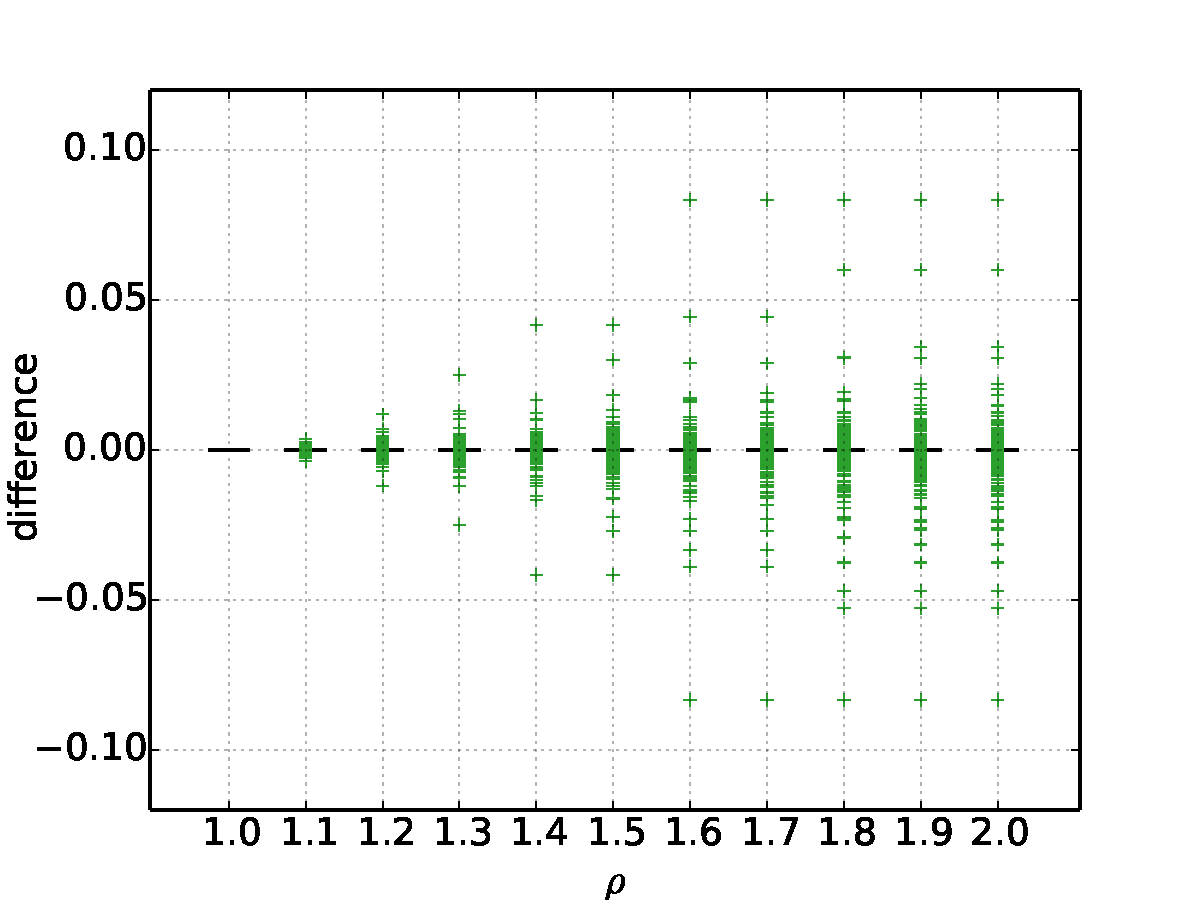
\includegraphics[width=0.49\textwidth]{figs/fig-score-variation-rr.pdf}
}
\subfloat[RBP0.5\label{fig-score-variation-rbp50}]{%
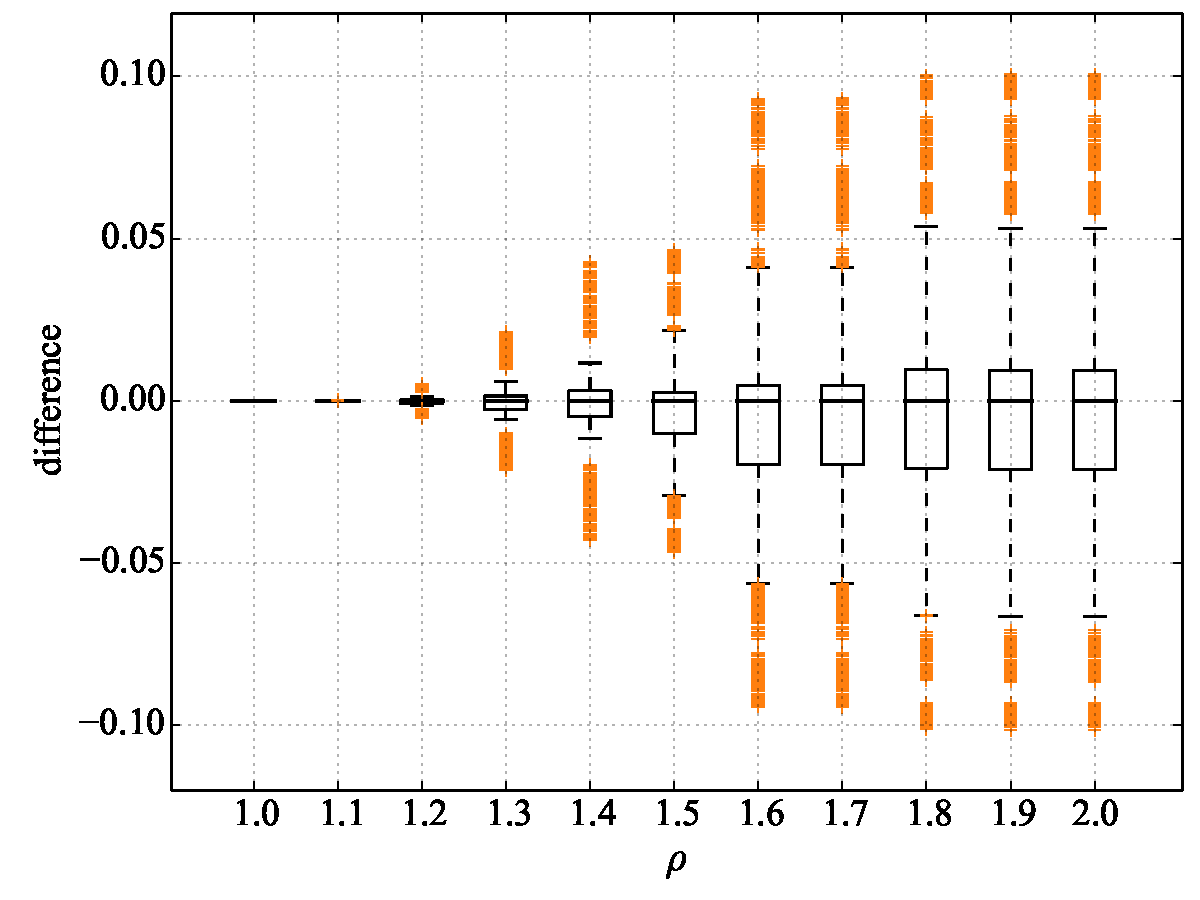
\includegraphics[width=0.49\textwidth]{figs/fig-score-variation-rbp50.pdf}
}
\\
\subfloat[RBP0.85\label{fig-score-variation-rbp85}]{%
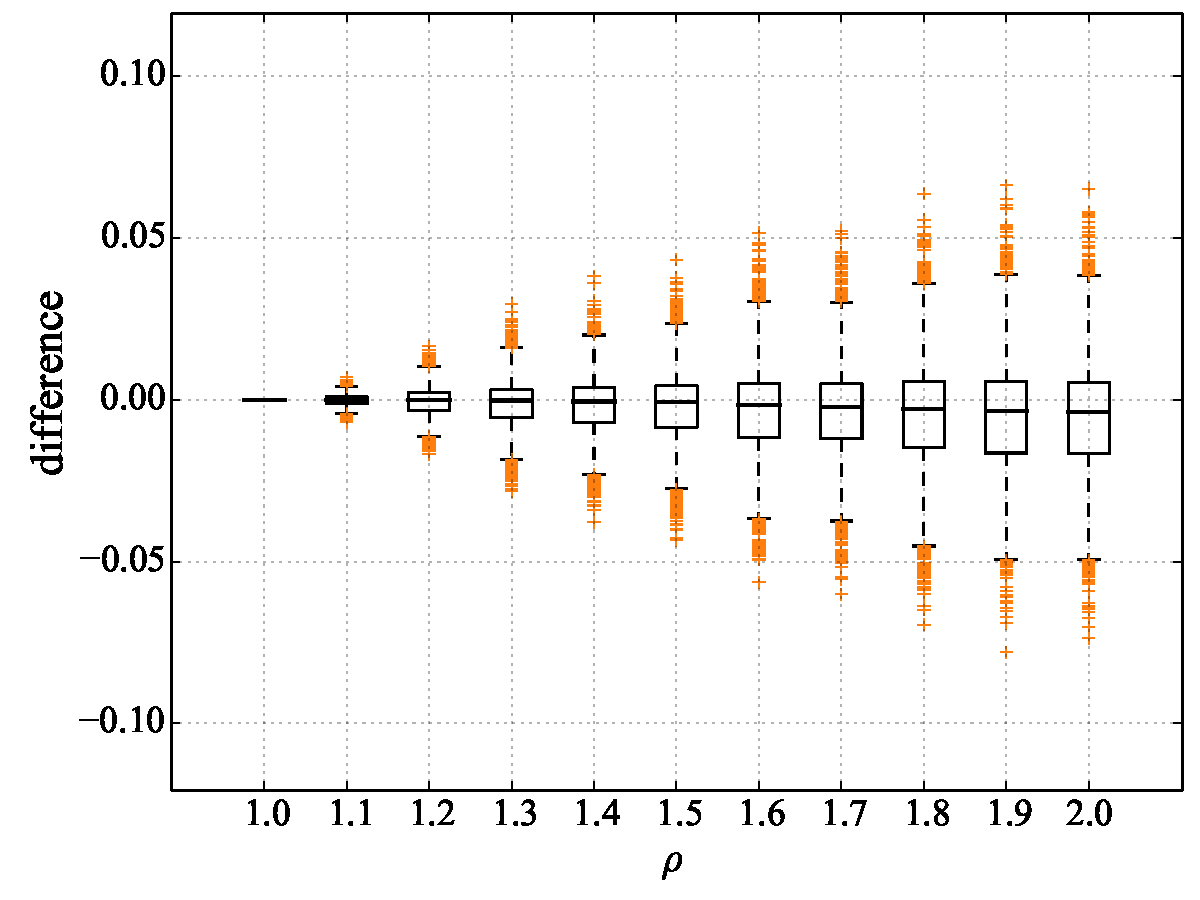
\includegraphics[width=0.49\textwidth]{figs/fig-score-variation-rbp85.pdf}
}
\subfloat[AP\label{fig-score-variation-ap}]{%
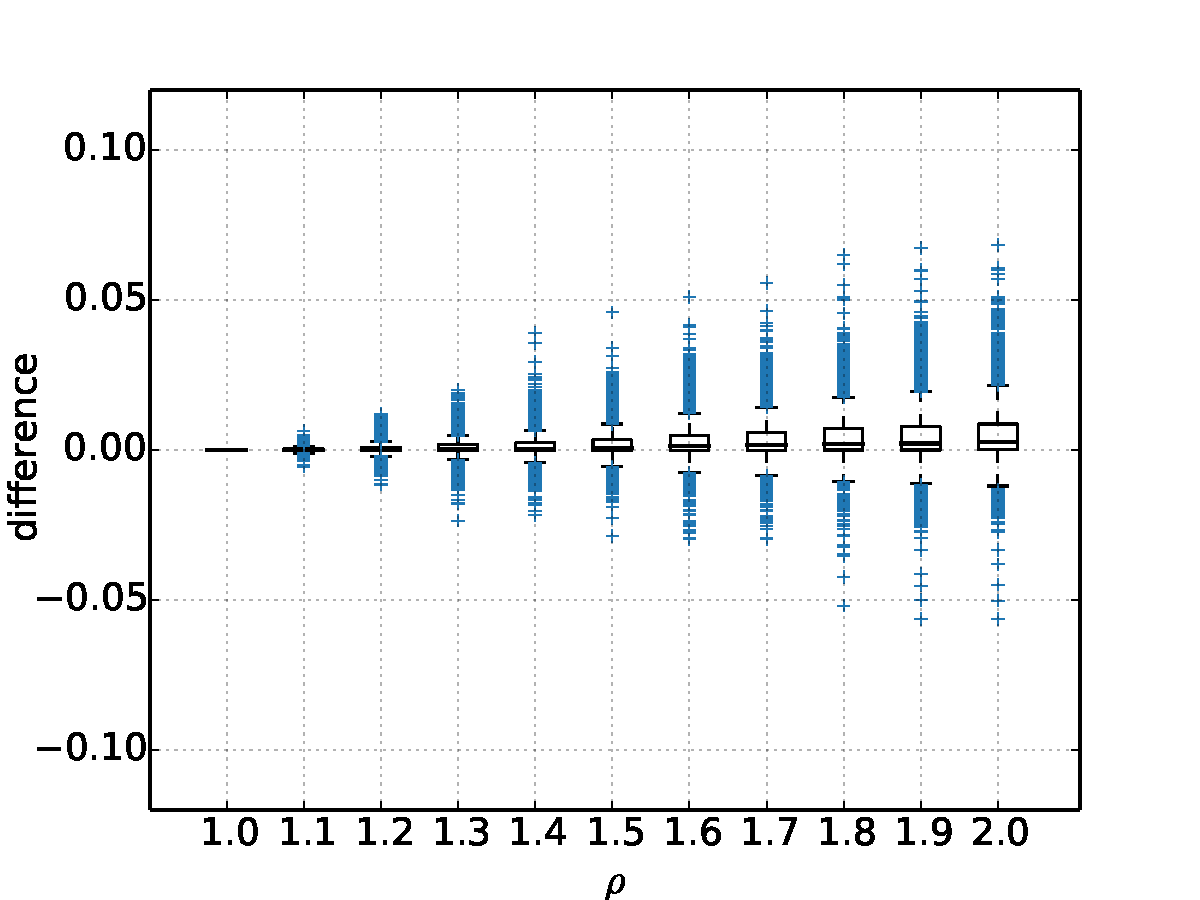
\includegraphics[width=0.49\textwidth]{figs/fig-score-variation-ap.pdf}
}
\caption{Variation in metric effectiveness score across a set of $98$
runs and $50$ topics (that is, $50 \times 98$ points are plotted in
each column), as a function of $\rho$, for four different retrieval
effectiveness metrics.
The whiskers indicate the last outlier still within $1.5$ of the
inter-quartile range from the corresponding quartlie (the limits of
the boxes), and then further outliers are plotted as separate colored
points.
\label{fig-score-variation}}
\end{figure}

Figure~\ref{fig-score-variation} shows the results of this
experimentation, plotted as a sequence of box-whisker elements using
four different effectiveness metrics and eleven values of $\rho$.
In all cases the score difference calculated is the
across-permutations computation that was illustrated in
Section~\ref{sec-ties} when applied to the deliberately-tied
rankings, subtracted from the score the same metric achieved on the
original submitted ranking for that same topic.
%% (We used a modified version of {\tt{trec\_eval}} to ensure that this
%% was done consistently.)
We followed standard protocols and assumed that unjudged documents
were not relevant for the purposes of scoring the runs.

Figure~\ref{fig-score-variation} shows that the average score
variation arising from the banding process is small, and that there
are nearly as many system-topic combinations that gain from the
approximation process as there are that lose from it.
Most RR values are unaffected (both quartiles are zero, for all of
the $\rho$ values tested), and the two deep metrics (RBP$0.85$ and
AP) also have small inter-quartile ranges on the computed score
differences.
The average original metric scores across all system-topic
combinations for RR, RBP0.5, RBP0.85, and AP are, respectively,
$0.6977$, $0.5610$, $0.4731$, and $0.2341$; and hence the fact that
the AP score differences are smaller than the score differences for
the other three metrics is in part a matter of relative scale.
The shallow metric RBP0.5 suffers the most from the score grouping
process; even so, it is only when $\rho>1.5$, the first value for
which ranks $2$ and $3$ are placed in the same group, that the
difference becomes large.
In all cases in which $\rho\le2$ the first group contains only a
single document.

\begin{table}[t!]
\centering
\renewcommand{\tabcolsep}{0.5em}
\newcommand{\tabent}[1]{\makebox[9mm][c]{#1}}
\begin{tabular}{l c cccc c cccc}
\toprule
\multirow{2}{*}{$\rho$}
	&& \multicolumn{4}{c}{Relative to $99$\% of original score}
		&& \multicolumn{4}{c}{Relative to $97$\% of original score}
\\
\cmidrule{3-6}\cmidrule{8-11}
	&& \tabent{RR}
		& \tabent{RBP0.5}
			& \tabent{RBP0.85}
				& \tabent{AP}
					&& \tabent{RR}
						& \tabent{RBP0.5}
							& \tabent{RBP0.85}
								& \tabent{AP}
\\
\midrule
1.1
	&& 80
		& 80
			& 80
				& 80
					&& 80
						& 80
							& 80
								& 80
\\
1.2
	&& 80
		& 80
			& 80
				& 80
					&& 80
						& 80
							& 80
								& 80
\\
%% 1.3
%% 	&& 80
%% 		& 79
%% 			& 76
%% 				& 73
%% 					&& 80
%% 						& 80
%% 							& 80
%% 								& 80
%% \\
1.4
	&& 77
		& 44
			& 65
				& 44
					&& 80
						& 80
							& 80
								& 80
\\
%% 1.5
%% 	&& 73
%% 		& 40
%% 			& 44
%% 				& 7
%% 					&& 80
%% 						& 80
%% 							& 80
%% 								& 80
%% \\
%% 1.6
%% 	&& 38
%% 		& 11
%% 			& 15
%% 				& 1
%% 					&& 80
%% 						& 67
%% 							& 80
%% 								& 80
%% \\
%% 1.7
%% 	&& 37
%% 		& 11
%% 			& 14
%% 				& 0
%% 					&& 80
%% 						& 67
%% 							& 80
%% 								& 77
%% \\
%% 1.8
%% 	&& 38
%% 		& 10
%% 			& 5
%% 				& 0
%% 					&& 80
%% 						& 61
%% 							& 77
%% 								& 60
%% \\
%% 1.9
%% 	&& 39
%% 		& 10
%% 			& 3
%% 				& 0
%% 					&& 80
%% 						& 61
%% 							& 72
%% 								& 43
%% \\
2.0
	&& 38
		& 10
			&\D3
				&\D0
					&& 80
						& 61
							& 71
								& 20
\\
\bottomrule
\end{tabular}

\caption{Number of systems (maximum $75$) for which a $t$-test across
$50$ topics yields confidence at the $p\le0.05$ level that the
grouped runs yield a metric score greater than or equal to $99$\% of
the original run score.
\label{tbl-frac-significant}}
\end{table}

%% \begin{figure}[t!]
%% \centering
%% \subfloat[RR\label{fig-rho-p-value-rr}]{%
%% 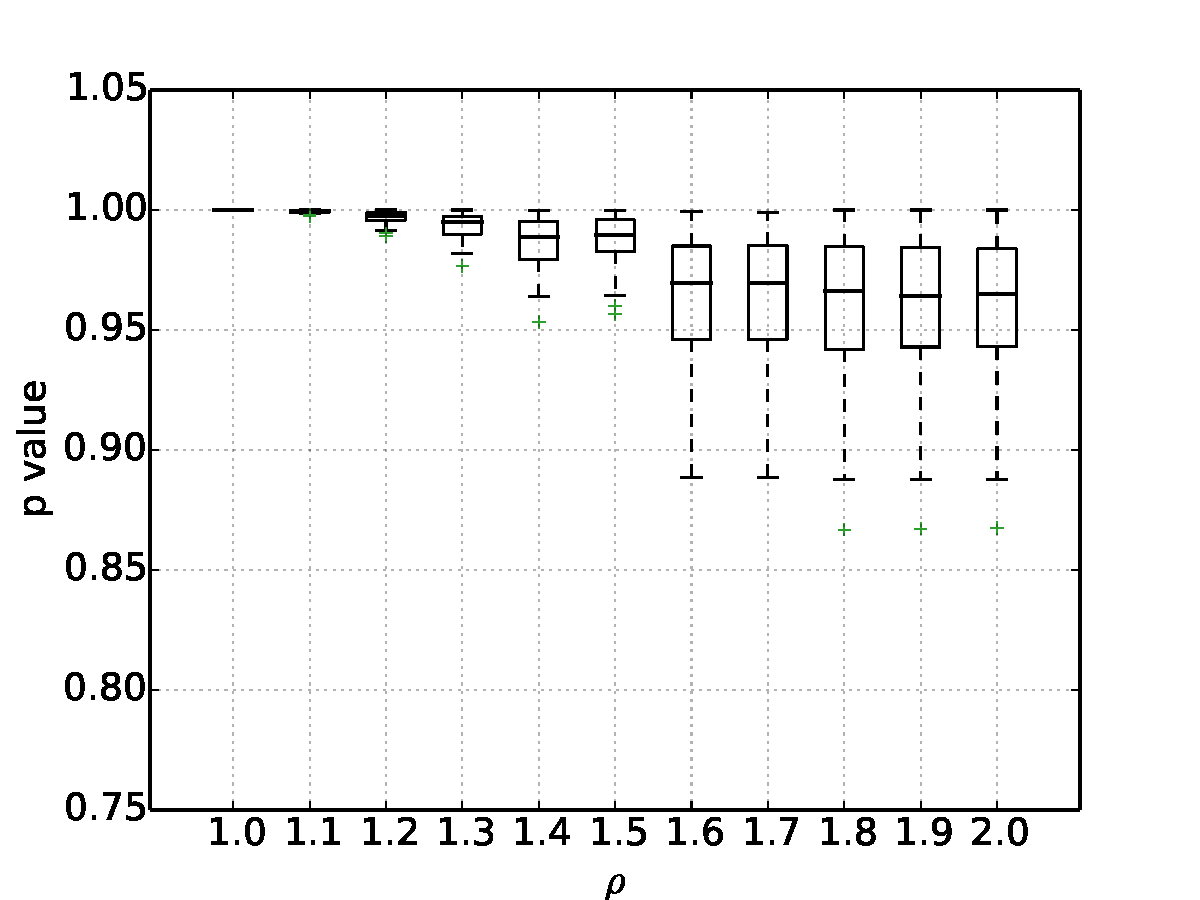
\includegraphics[width=0.49\textwidth]{figs/fig-rho-p-value-rr.pdf}
%% }
%% \subfloat[RBP0.5\label{fig-rho-p-value-rbp50}]{%
%% 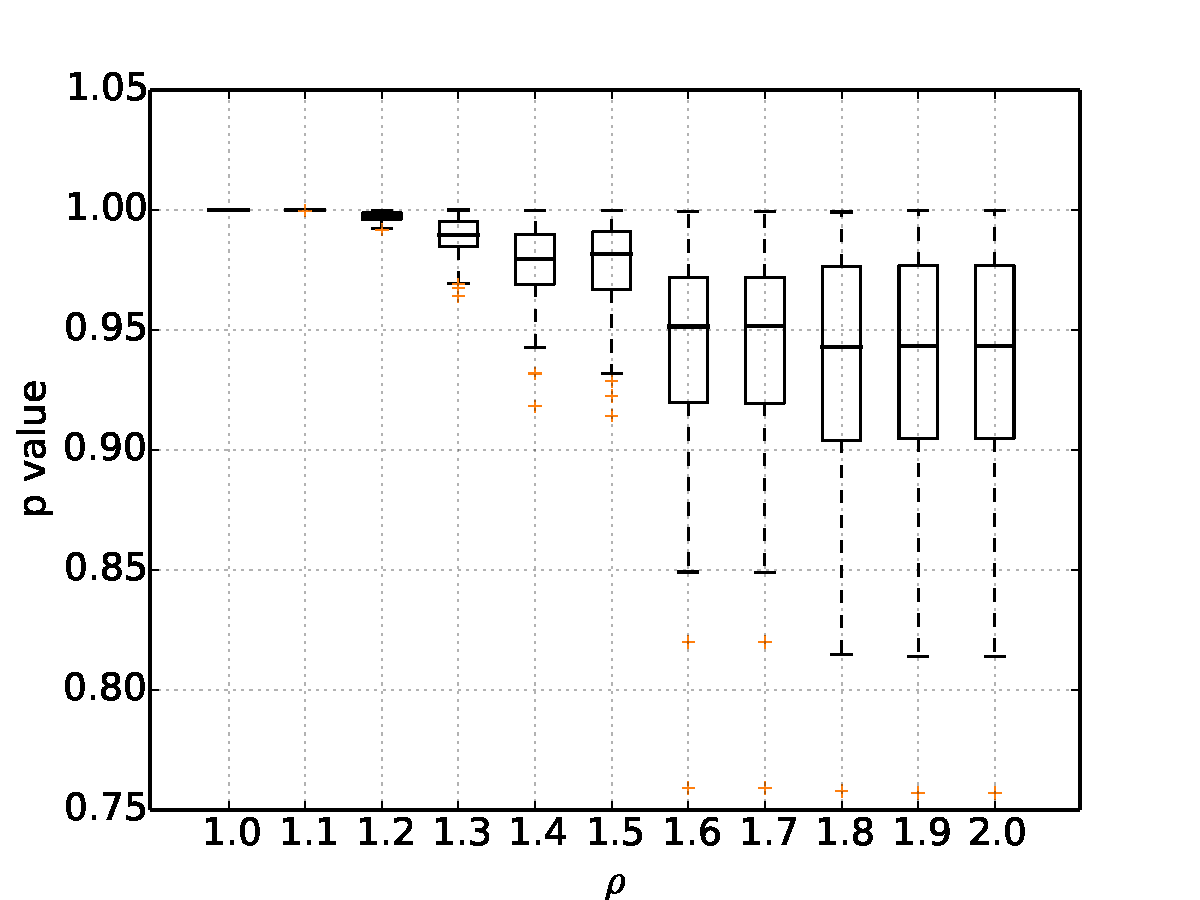
\includegraphics[width=0.49\textwidth]{figs/fig-rho-p-value-rbp50.pdf}
%% }
%% \\
%% \subfloat[RBP0.85\label{fig-rho-p-value-rbp85}]{%
%% 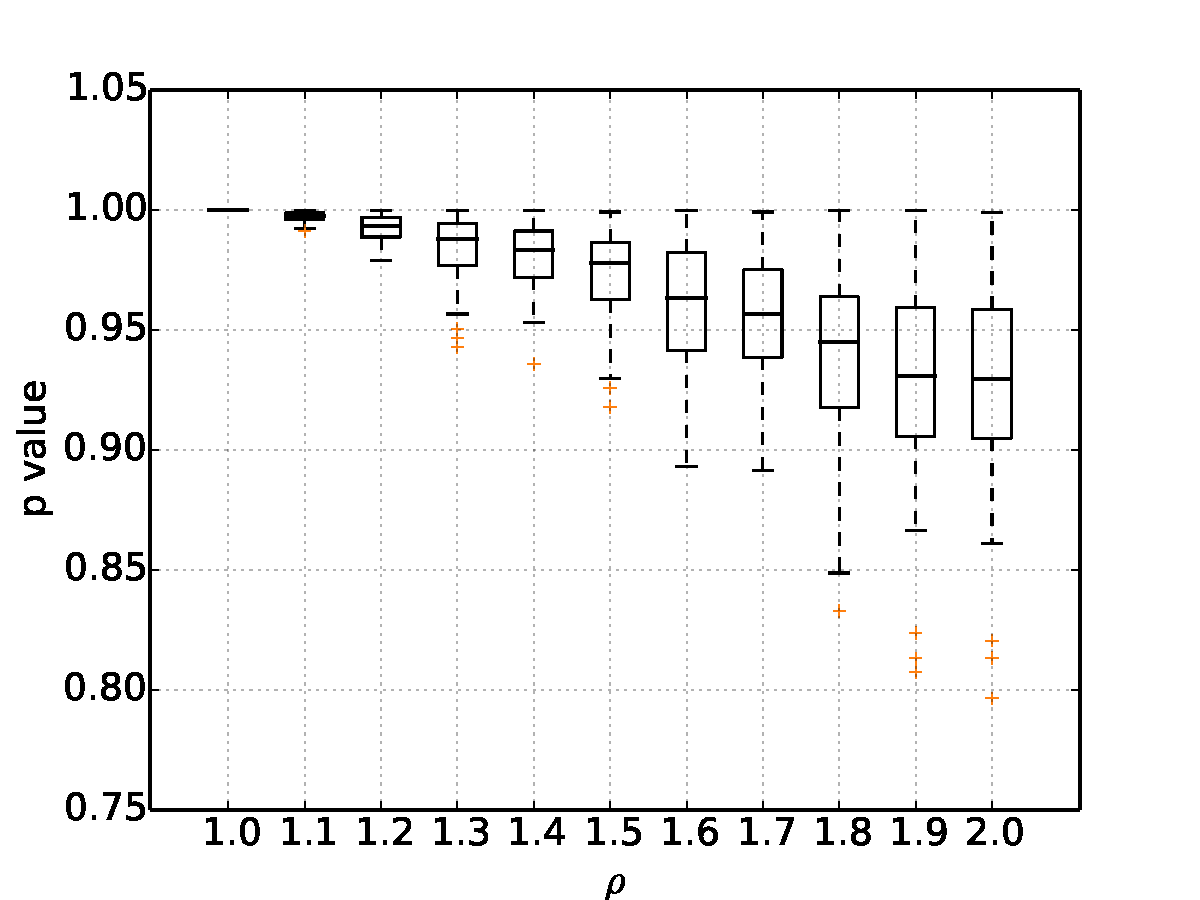
\includegraphics[width=0.49\textwidth]{figs/fig-rho-p-value-rbp85.pdf}
%% }
%% \subfloat[AP\label{fig-rho-p-value-ap}]{%
%% 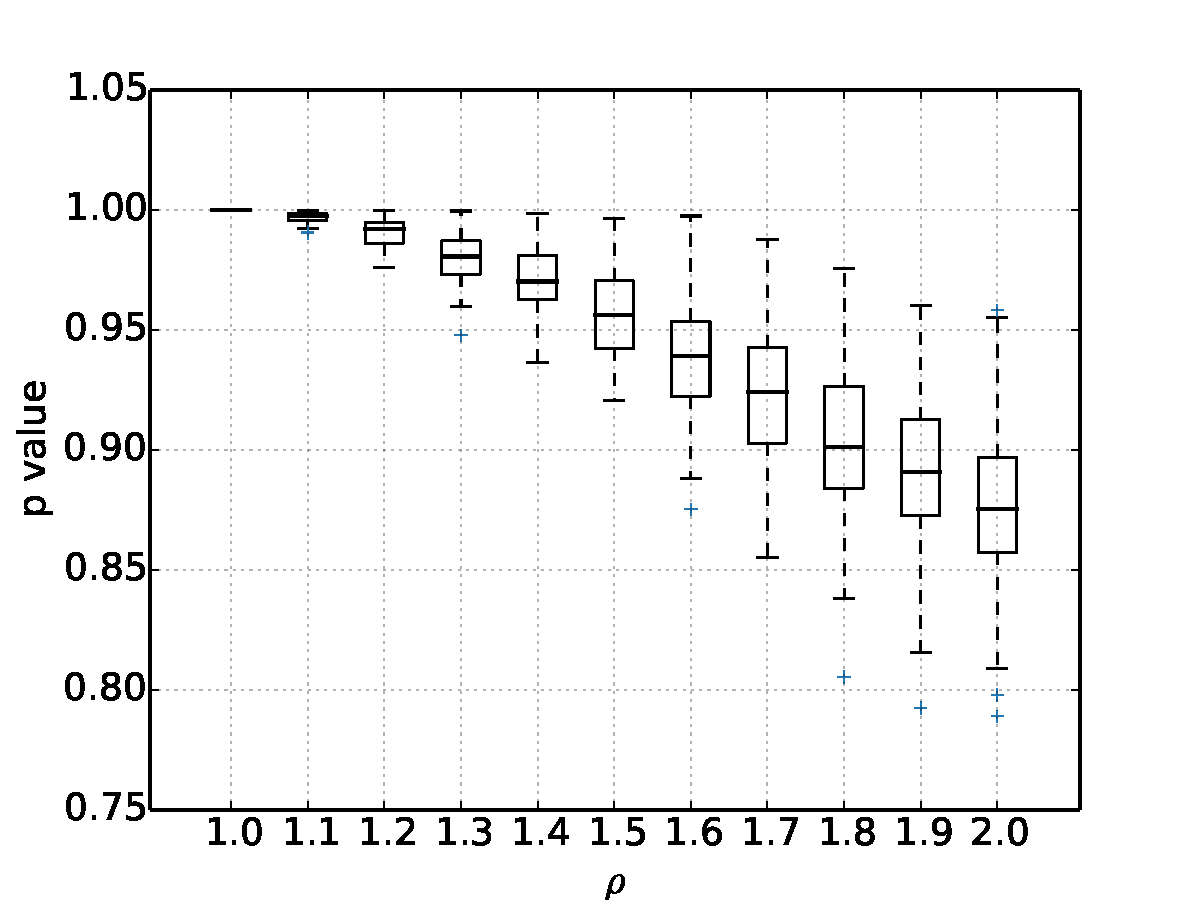
\includegraphics[width=0.49\textwidth]{figs/fig-rho-p-value-ap.pdf}
%% }
%% \caption{Distribution of two-tailed $t$-test $p$ values generated by
%% comparing system scores for $98$ original-order runs, and the
%% corresponding set of $98$ grouped-score runs ($98$ points plotted in
%% each column), in each case over a set of $50$ topic scores.
%% A $p$ value of $1.0$ indicates that the two sets of rankings have
%% identical means across the $50$ topics.
%% \label{fig-rho-p-value}}
%% \end{figure}
%% 
%% Figure~\ref{fig-rho-p-value} explores whether these small score
%% differences can be regarded as being significant.

Table~\ref{tbl-frac-significant} explores whether the small score
differences identified in Figure~\ref{fig-score-variation} can be
regarded as being significant.
To generate the table, each of the $75$ systems was scored for the
$50$ topics using the original runs, and then rescored using the
grouped runs.
The set of original topic scores was then multiplied by $0.99$, and
compared to the grouped scores, using a one-tail paired $t$-test.
If a $p$ value less than or equal to $0.05$ was generated by that
test, that system was counted as being one for which the grouping
process degraded the system score by $1$\% or less.
The closer the count of such systems is to $75$, the greater the
confidence we can have that the grouping process will not give
notably inferior system scores overall, where ``notably inferior'' is
defined (here) as being a $1$\% degradation in measured score.

As can be seen, {\alistair{more...}}

%% {\alistair{If still don't like the idea of having $p\approx1$
%% indicating the two distributions have the same mean, can change tack,
%% and ask (positive) question, ``is treated run scoring $>0.99$ of
%% original run scoring''.
%% Then small $p$ values indicate confidence that the treatment (ie,
%% grouping) achieves effectiveness within (or greater than) one percent
%% of the original system.}}
%% 
%% {\andrew{all possible 1024 of length 10?}}
%% {\andrew{I still don't like not being able to see the original metric value. 
%% What is a difference of 0.1 compared to the original values?}}

\myparagraph{System Comparison Sensitivity}

Effectiveness measurements are also used to compare systems in a
pairwise manner.
In the second experiment, we explore the implications that score
rounding has on the ability of metrics to differentiate between
systems.
The normal approach to comparing systems is to take their computed
scores across a set of topics, and perform a paired $t$-test to
explore the null hypothesis that the two systems are in fact the
same.
The process of carrying out the $t$-test generates a $p$ value; the
smaller the $p$ value, the smaller the chance that the two systems
being compared are giving the same performance.
To establish significance, a threshold value $\alpha$ is employed,
often $\alpha=0.05$, with $p\le\alpha$ being regarded as a
significant outcome.

\begin{figure}[t!]
\centering
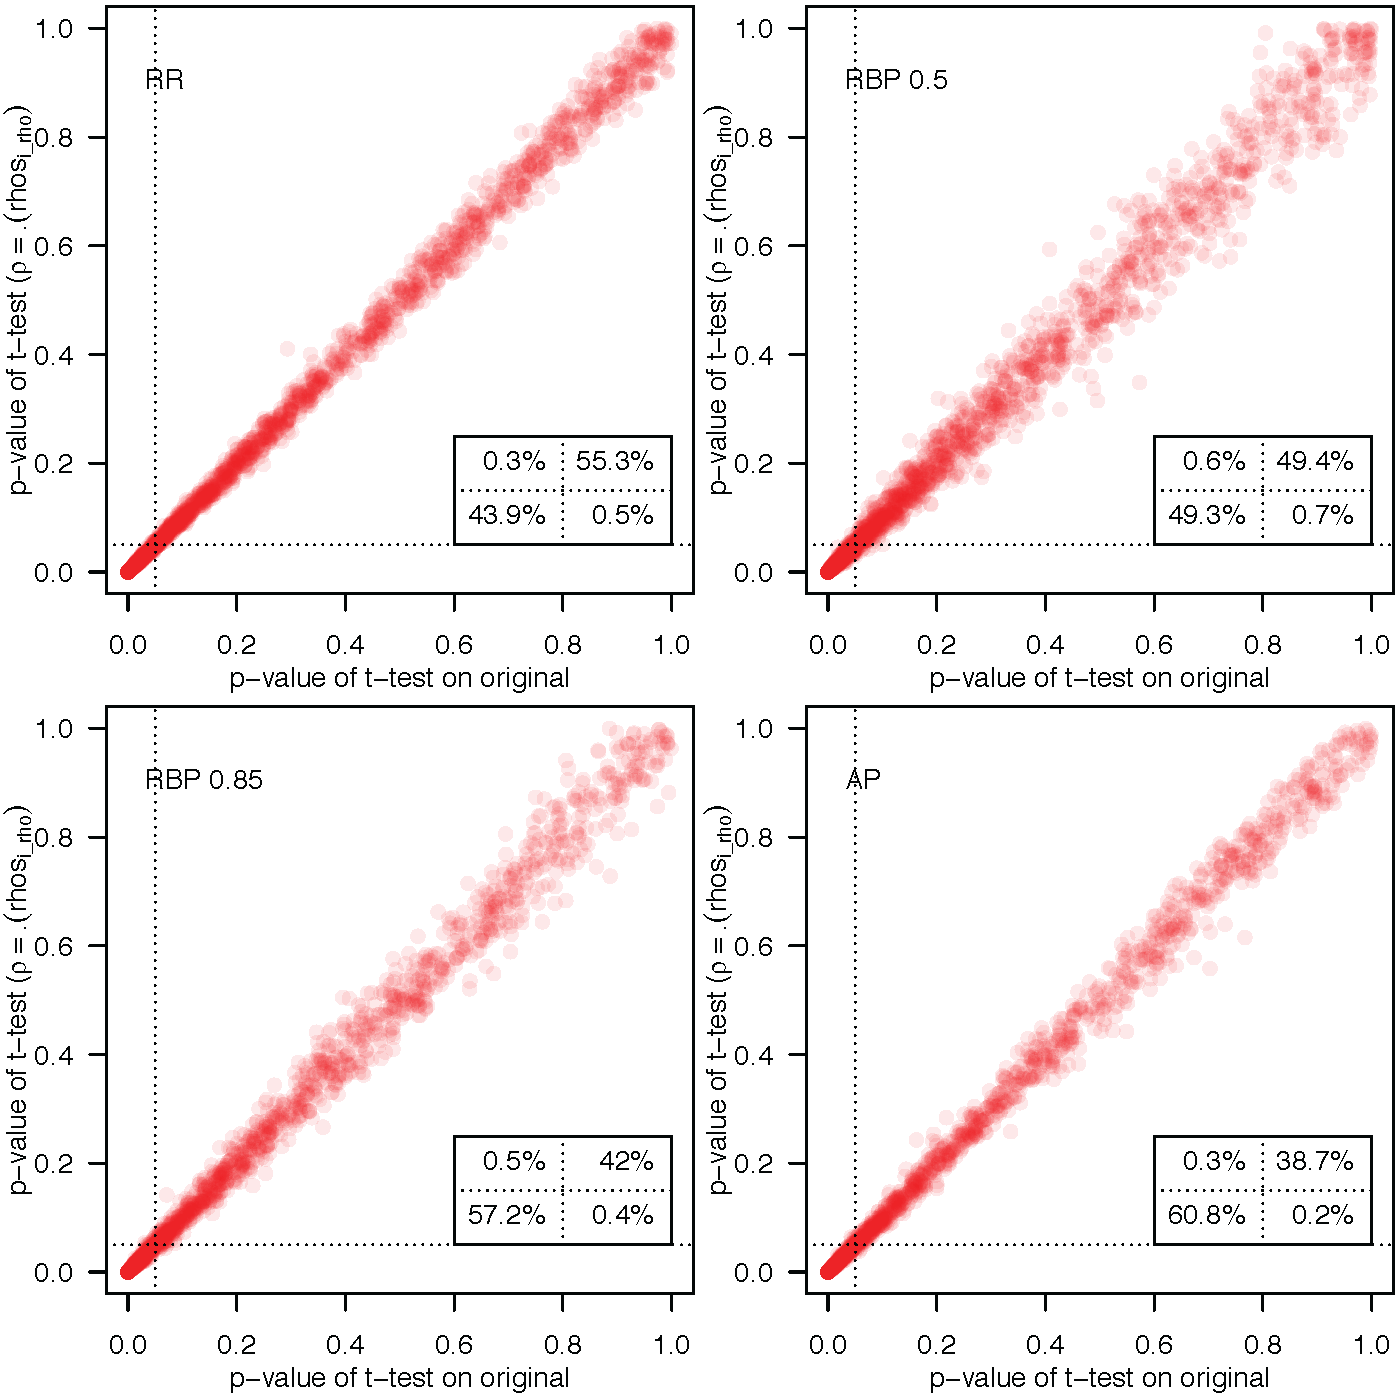
\includegraphics[width=0.98\textwidth]{tmp-fig-03.png}
\caption{Correlation of $p$ values for all pairs of systems
($75\times74/2=2775$ points per pane), with the $p$ value from a
$t$-test using the original system scores across $50$ topics plotted
on the horizontal axis, and the $p$ value for the corresponding
grouped run for on the vertical axis, using $\rho=1.5$ throughout.
The dotted lines mark the $p=0.05$ regions, with the grid of values
showing the percentage of data points falling in each quadrant.
\alistair{Temporary figure, one frame stolen out of Andrew's PDF file.}
\label{fig-pair-variation}}
\end{figure}

To measure the effect that score rounding has on system comparisons,
we took the $50$ topics of the TREC7 collection and the $98$ runs
associated with it that we have been using, and computed, for each of
eleven different values of $\rho$, the set of $p$ values generated
for the $98\times97/2$ distinct system pairs.
In all cases when $\rho>1$, the averaging processes described in
Section~\ref{sec-ties} were ued; when $\rho=1$, each run was
processed in run order, and the supplied scores were ignored.

Figure~\ref{fig-pair-variation} shows {\alistair{more...}}
